\newpage
\subsubsection{Module d'exploitation des données}
\begin{figure}[h!]  
  \centering
    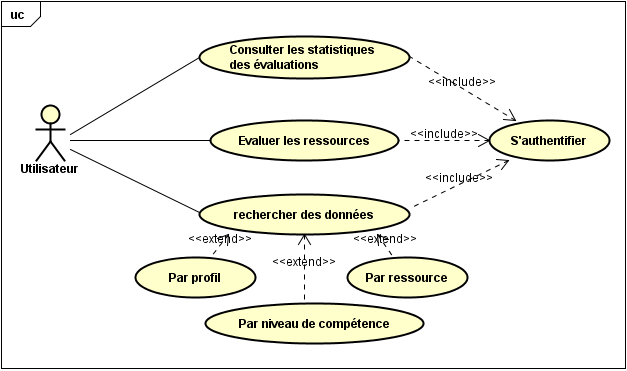
\includegraphics[width=0.95\textwidth]{chapitre2/Figures/competencesUC.png}
  \caption{Diagramme de cas d’utilisation du module de la matrice de comptétences}
\end{figure}
\subsubsection*{Description des cas d’utilisations }
\begin{itemize}[label=\textbullet]
\newpage
%Consulter l'état matériel
\item \textbf{Consulter l'état d'un TPE :}
\begin{table}[!h]
\begin{tabular}{|p{15cm}|}%p{2.5cm}|p{9cm}
\rowcolor{shadecolor}\multicolumn{1}{|c|}{Sommaire d’indentification} \\
\hline
\textbf{objectif : } cette fonctionnalité permet de visualiser les informations concernant l'état en temps réel du TPE \\
\textbf{acteurs : } utilisateur\\
\textbf{précondition : } 
	\begin{itemize}[label=\textbullet]
	\item l'acteur est connecté au système
	\item l'acteur a le droit d'accès
	\end{itemize}
	\\
\hline
\rowcolor{shadecolor}\multicolumn{1}{|c|}{Description des scénarios} \\
\hline
	\textbf{Scénario nominal :}
	\begin{itemize}[label=\textbullet]
	\item scénario "Consulter l'état d'un TPE" :
		\begin{itemize}
		\item l'acteur demande de visualiser les informations de l'état du TPE
		\item le système regroupe l'ensemble des informations demandées 
		
		\item le système affiche les informations du TPE et des tableaux qui synthétise l'état matériel et logiciel du TPE
		\end{itemize}
	\end{itemize}
	\\
\hline
\end{tabular}
\centering \caption{Description du cas d’utilisation "Consulter l'état d'un TPE"} \label{TablePR}
\end{table}



\newpage
%Consulter les statistiques d'un groupe de TPE
\item \textbf{Consulter les statistiques d'un groupe de TPE :}
\begin{table}[!h]
\begin{tabular}{|p{15cm}|}%p{2.5cm}|p{9cm}
\rowcolor{shadecolor}\multicolumn{1}{|c|}{Sommaire d’indentification} \\
\hline
\textbf{objectif : } cette fonctionnalité permet de visualiser  les statistiques d'un groupe de TPE \\
\textbf{acteurs : } utilisateur\\
\textbf{précondition : } 
	\begin{itemize}[label=\textbullet]
	\item l'acteur est connecté au système
	\item l'acteur a le droit d'accès
	\end{itemize}
	\\
\hline
\rowcolor{shadecolor}\multicolumn{1}{|c|}{Description des scénarios} \\
\hline
	\textbf{Scénario nominal :}
	\begin{itemize}[label=\textbullet]
	\item scénario "Consulter les statistiques d'un groupe de TPE" :
		\begin{itemize}
		\item l'acteur sélectionne un groupe de TPE
		\item le système affiche la liste des TPE et des champs de dates et de choix d'unité de temps
		\item l'acteur sélectionne : l'ensemble des TPE,date début, date fin, l'unité de temps(jours,mois)
		\item l'acteur lance la recherche
		\item le système affiche des champs, tableaux et des graphes qui synthétisent l'ensemble des statistiques.
		\end{itemize}
	\end{itemize}
	\\
\hline
\end{tabular}
\centering \caption{Consulter les statistiques d'un groupe de TPE"} \label{TablePR}
\end{table}



\end{itemize}
